\section{Płatności elektroniczne}
Coraz częściej urządzenia mobilne pośredniczą w opłatach za przedmioty codziennego użytku. Można w taki sposób zapłacić w sklepie, bądź kupić bilet w komunikacji miejskiej. Realizacja tego typu transakcji odbywa się drogą elektroniczną, z wykorzystaniem płatności elektronicznych. W tym rozdziale zostaną one opisane oraz poddane analizie.

\subsection{Wprowadzenie}

Bardzo często e-commerce niepoprawnie utożsamiany jest tylko z dokonywaniem zakupów przez internet, mimo że może odbywać się także z wykorzystaniem m.in.~telefonu, faksu, czy telewizji. Odnosi się ogólnie do stosowania urządzeń elektronicznych w zakupie oraz sprzedaży. Jednak to właśnie internet jest dominującą obecnie formą e-handlu, będąc medium informacyjnym łączącym niejako wszystkie poprzednio używane. Jego nieograniczone możliwości przyciągają nowych użytkowników, którzy z czasem nabierają zaufania i stają się także kupującymi. W ten sposób dynamiczny rozwój sieci napędza także handel elektroniczny. Przedsiębiorcy chcąc zachować kontakt z klientami muszą zaznaczyć swoją obecność tam, gdzie koncentruje się coraz większa część ludzkiej aktywności. Owocuje to powstawaniem nowych sklepów internetowych.

Tradycyjne formy przeprowadzania transakcji nie pasują do specyfiki biznesu internetowego. Opłata za pobraniem związana jest z wyższą prowizją, a przelewy wiążą się z długim czasem oczekiwania na zrealizowanie operacji finansowej. Nie są to efektywne metody płatności w internecie, gdzie niebagatelne znaczenie ma właśnie szybkość. Alternatywą, a także odpowiedzą na oczekiwania e-biznesu, są należące do bezgotówkowych form transakcji - płatności elektroniczne. Są to wszelkiego rodzaju opłaty, zawierane za pośrednictwem internetu. Nazywane także e-płatnościami \cite{elektroniczne_metody_platnosci}, przeprowadzane są różnymi kanałami elektronicznymi, do których należą: karty płatnicze, czy przelewy bankowe. Bardzo popularne są ostatnio także usługi oferowane przez dostawców płatności elektronicznych, takich jak PayPal. Realizacja e-płatności wymaga posiadania urządzenia elektronicznego, do których zaliczają się: komputery, tablety i smartfony. 

Handel internetowy nie mógł by istnieć bez płatności internetowych. To właśnie wspólny rozwój e-handlu z internetem umożliwił powstanie nowej metody zawierania transakcji. Dzięki temu są one dobrze przystosowane do wymagań stawianych w rozwiązaniach z dziedziny e-commerce. Oprócz szybkości, oferują one także bezpieczeństwo oraz wygodę w zawieraniu transakcji. Dzięki coraz większej konkurencji pomiędzy dostawcami usług płatniczych - także korzystniejsze prowizje. Ich zastosowanie rośnie, wraz z rosnącą liczbą usług oferowanych w internecie. Szczególnie zaznaczyły swoja obecność w aplikacjach mobilnych. Opłaty mogą być związane z uzyskaniem dostępu do takiego programu, bądź dodatkowej treści.

Po kilkunastu latach płatności elektroniczne dalej są w fazie dynamicznego rozwoju. Dzięki rozwojowi technologii znajdują się dla nich cały czas nowe zastosowania. 


\subsection{Ewolucja systemów płatniczych}

Płatności elektroniczne mają swój początek w e-bankowości. Wprowadzanie przez banki, a później instytucje pozabankowe, nowe udogodnienia technologiczne, spowodowały radykalną zmianę w sposobie przeprowadzania operacji finansowych. Przykładem tego mogą być karty płatnicze, zaprezentowane po raz pierwszy w latach pięćdziesiątych. Innym znaczącym osiągnięciem są pieniądze elektroniczne, także będące formą bezgotówkowych transakcji. 

\subsubsection*{Bankowość elektroniczna}

Bankowość elektroniczna kryje się pod wieloma nazwami: Internet banking, e-banking, on-line banking. Według J. Masiota jest to ``każda usługa bankowa, która umożliwia klientowi wzajemny kontakt z instytucją bankową z oddalonego miejsca poprzez: telefon, terminal, komputer osobisty, odbiornik telewizyjny z dekoderem'' \cite{pieniadz_elektroniczny-analiza}. Dodatkowo użytkownikowi oferowany jest podobny zakres usług jak w placówce fizycznej. Ogólnie dotyczy ona zdalnej obsługi konta bankowego. Pierwsze zastosowanie e-bankingu nastąpiło w USA, gdzie Diners Club wprowadził kartę płatniczą \cite{pieniadz_elektroniczny-analiza}. Nikt wtedy nie mógł zdawać sobie sprawy, jaką wielką popularność zyska ten instrument płatniczy. Następnie w 1970 r. powstał system kart debetowych, a w latach osiemdziesiątych pojawiły się  karty zawierające mikrochip. W Polsce pierwsze bankomaty powstały w 1990~r. za sprawą banku Pekao~S.A.

Home banking był jedną z form bankowości elektronicznej, który powstał z myślą o klientach indywidualnych i małych przedsiębiorcach. Po zainstalowaniu specjalnego oprogramowania, bądź kupienia odpowiedniej przystawki, klient mógł wykonywać operacje na swoim koncie. Ta i podobne odmiany e-bankingu nie zdążyły na dobre zaznaczyć swojej obecności. Wprowadzenie internetu do powszechnego użytku, przemodelowało dotychczas stosowane rozwiązania.

\subsubsection*{Bankowość internetowa}

Początki sieci globalnej sięgają lat sześćdziesiątych XX stulecia, kiedy to na zlecenie Departamentu Obrony USA opracowany został ARPA-Net \cite{pieniadz_elektroniczny-analiza}. Od tego momentu Internet ewoluował, modyfikując stopniowo naszą rzeczywistość. Duże ułatwienia w komunikowaniu się wpłynęły na przemiany społeczne, oprócz tego powstanie oraz rozwój sieci odbił się szczególnie mocno na dziedzinach związanych z przetwarzaniem informacji \cite{pieniadz_elektroniczny-analiza}, czyli m.in. na sektor bankowy. Jego podatność na innowacje technologiczne pozwoliła na zupełnie nowy sposób dostępu do usług bankowych.

W bankowości internetowej oraz wirtualnej komunikacja odbywa się za pośrednictwem przeglądarki internetowej. Klient ma dostęp do większości usług oferowanych przez bank w placówce. Użytkownik może kontrolować stan konta, zaciągać kredyty lub wykonywać przelewy. Dostępność do takiej usługi jest niezależna od miejsca, 24 godziny na dobę i posiada wszystkie zalety, jakie niesie ze sobą korzystanie z internetu. La Jolla Bank FSB w 1994~r. był pierwszym bankiem, który umożliwił wykonywanie podstawowych operacji za pośrednictwem sieci. Ciekawą i dość popularną także w Polsce odmianą bankowości, jest bankowość wirtualna. Polega ona na obsłudze klienta tylko internetowo, a banki takie często nie posiadają nawet swoich placówek. Przykładem takich banków jest chociażby mBank. 

Sieć, by móc się rozprzestrzeniać, musiała przez lata wykształcić takie właściwości, jak: bezpieczeństwo, uniwersalność, interaktywność. Chcąc dokonać płatności, czy sprawdzić konto w banku chcemy mieć pewność, że nasze dane są bezpieczne. Istotny jest także sposób dostępu, coraz mniej zależny od używanego systemu operacyjnego. Na przestrzeni lat najważniejszy okazał się jednak stały rozwój. 

\subsubsection*{Pierwsza generacja płatności internetowych}

Rozpoczęta w latach dziewięćdziesiątych pierwsza generacja płatności, próbowała wprowadzić alternatywną gotówkę, np.: e-monety, czy tokeny \cite{elektroniczne_metody_platnosci}. E-gotówka miała zachować wszystkie cechy tradycyjnego pieniądza, oferując m.in. brak opłat transakcyjnych, czy anonimowość. Pierwszym systemem był wydany w 1994 r. e-cash, założony przez amerykańską firmę DigiCash. Podobnie jak w większości wprowadzanych w tamtym czasie rozwiązań, tak samo e-cash oznaczał elektroniczną walutę indywidualnym numerem seryjnym. Takie podejście miało chronić pieniądze przed fałszerstwem, a dostarczało tylko dodatkowych trudności. Cechą wspólną pierwszej generacji jest trudność w obsłudze oraz wymaganie dodatkowego oprogramowania, bądź nawet czytników kart. Sama firma DigiCash zakończyła swoją działalność w 1998 r.

\subsubsection*{Druga generacja płatności internetowych}

Trwająca do dziś i charakteryzująca się znacznie większą prostotą druga generacja, została zapoczątkowana na przełomie XX i XXI wieku. Jej powstanie i odmienność od wcześniej stosowanych rozwiązań, wynika z możliwości i ułatwień jakie posiada internet. Po kilkunastu latach dynamicznego rozwoju, zdążył się lepiej dostosować do stawianych mu wymagań. Szczególnie postęp do obszarze zabezpieczeń, wiążący się z powstaniem szyfrowanych protokołów przesyłania danych (np.: HTTPS), jest znaczący w systemach płatności. Nie są już potrzebne specjalne czytniki, wszystko może odbywać się przez przeglądarkę internetową. Sprawia to, że korzystanie z takiej formy płatności jest znaczenie wygodniejsze i szybsze, a także prostsze, gdyż zmniejsza się ilość kroków, jakie trzeba wykonać, aby dokonać zakupu. Lepsza edukacja oraz coraz dłuższe przebywanie w sieci sprawia, że ludzie częściej będą się decydować na tę formę płatności.  


\subsection{Analiza metod płatności}

Różnorodność dostępnych metod płatności internetowych sprawia, że mogą być one bardzo dobrze wpasowane w każdy model biznesowy. Ważnym kryterium przy wyborze płatności jest wielkość pojedynczej transakcji w systemie, co wiąże się bezpośrednio z poziomem zabezpieczeń jaki należy zapewnić. Na decyzję powinny także wpływać indywidualne preferencje użytkowników. Nie warto kierować się tylko wygodą, czy innowacyjnością. Szczególnie istotny jest poziom zaufania, z jakim spotyka się dane rozwiązanie. Duża część użytkowników internetu przyzwyczajona jest do tradycyjnych płatności, szczególnie do gotówki i takiej formy zapłaty będą oczekiwać. Jest to ważny wybór, wpływający na odczucia płynące z korzystania z serwisu.

\subsubsection*{Wysokość transakcji}
Przedstawiony poniżej podział, dokonany został ze względu na wielkość pojedynczej transakcji. Obok każdej z kategorii zostały podane wartości, z którymi można się w ich przypadku najczęściej spotkać. Niema w biznesie jednej, ścisłej definicji wymienionych tutaj typów płatności. Wartości mogą się też różnić, w zależności od dostawcy usług płatniczych. To rozróżnienie sugeruje przede wszystkim poziom zabezpieczeń, jaki należy zapewnić podczas przeprowadzania transakcji.
\begin{itemize}
	\item Milipłatności - płatność do kilkudziesięciu groszy,
	\item Mikropłatności - 1~zł do 80~zł,
	\item Minipłatności - 80~zł do 800~zł,
	\item Makropłatności - wszystko powyżej 800~zł. 
\end{itemize}
Milipłatności z mikropłatnościami dotyczą niewielkich, bardzo często kilkugroszowych operacji finansowych. Ich definicja różni się co do górnej granicy transakcji - najczęściej wynosi ok. 80 zł. Oprócz kwoty, dodatkowym wyróżnikiem jest krótki czas oraz łatwość w przeprowadzaniu płatności. Użytkownik spodziewa się, że taki proces nie będzie wymagał podjęcia przez niego wielu kroków - bardzo często opłaty w sklepach internetowych mogą być zrealizowane bez konieczności opuszczania strony sprzedającego. Ze względu na małe kwoty zabezpieczenia nie muszą być bardzo restrykcyjne, co pozwala na wprowadzenie wymienionych udogodnień. Większość transakcji zawieranych w internecie zamyka się w granicach mikropłatności. To właśnie ich dalszy rozwój, poprzez powstawanie nowych kanałów realizacji opłat, jest najistotniejszy zarówno dla sprzedawców jak i kupujących. Wydawnictwa coraz częściej decydują się na cyfrową dystrybucję książek, czy artykułów.

Podejście do zabezpieczeń w przypadku minipłatności musi być zdecydowanie bardziej rygorystyczne, a dla makropłatności stanowi to już priorytet. Tego typu transakcje związane są z większą liczbą kroków, jaką konsument musi wykonać, aby mogła być zrealizowana. Najczęściej będzie się odbywała za pośrednictwem strony banku lub dostawcy usług płatności. Powoduje to, że zakupy są znacznie wolniejsze, jednak w tym przypadku nie jest to wadą. Dzięki  temu ryzyko niechcianych zakupów lub dokonania transakcji przez osobę trzecią jest mniejsze. Płatności mogą dotyczyć np.: zakupu sprzętu RTV lub AGD.

\subsubsection*{Moment pobrania}
W przeciwieństwie do tradycyjnych metod płatności te elektroniczne mogą zostać w znaczenie większym stopniu dopasowane do potrzeb przedsiębiorstwa. To właśnie  elastyczność przyczynia się w znacznym stopniu do ich rozpowszechniania. Jednym z takich czynników jest właśnie moment pobrania. Dokonanie zakupu towaru bądź usługi, nie zawsze musi się wiązać z natychmiastowym pobraniem pieniędzy z konta. W zależności od rodzaju płatności elektronicznej, przelanie pieniędzy będzie odbywać na różnych etapach. Niektóre serwisy mogą na przykład wymagać zakupu wirtualnej waluty, obowiązującej tylko w jego ramach. Taka sytuacja często spotykana jest w grach sieciowych. 

Poniżej przedstawione zostały różne momenty pobrania, z jakimi można się spotkać w płatnościach elektronicznych. Wybór konkretnej kategorii będzie wiązał się z szybkością transakcji oraz poziomem zabezpieczeń, niezbędnym podczas ich realizacji.
\begin{itemize}
	\item System przedpłat (\textit{pay before}) - użytkownik najpierw musi zasilić swoje wirtualne konto, aby później mieć możliwość dokonywania zakupów.
	\item System natychmiastowych płatności (\textit{pay now}) - występuje w przypadku kart debetowych. Obciążenie rachunku następuje w momencie dokonania płatności. Nie ma możliwości uzyskania kredytu.
	\item System z odroczoną płatnością (\textit{pay later}) - do tego typu płatności należą karty kredytowe i obciążeniowe. Rachunek posiadacza takich instrumentów płatniczych zostanie obciążony, dopiero w momencie spłaty zaciągniętego kredytu.
\end{itemize}
%TODO przepisać, przenieść tutaj opisy poszczególnych momentów, pay-before w potaci portmonetek zostanie szczegółowo opisany niżej
Dużą popularność zyskują rozwiązania typu \textit{pay-before}. Funkcjonują one pod postacią wirtualnych portmonetek, gdzie użytkownicy trzymają elektroniczne pieniądze. Najpierw zasilone wpłaconą przez właściciela sumą, mogą być wykorzystywane do najróżniejszych transakcji finansowych. Są opcją szczególnie korzystną w przypadku częstych opłat, ponieważ nie są z nimi związane prowizje od każdej operacji, jak w przypadku kart. Także są względnie bezpieczniejsze - użytkownik nie łączy się za każdym razem z bankiem, a w przypadku oszustwa - nie przekroczy środków zgromadzonych na koncie.

\subsubsection*{Metody płatności w internecie}
Zakupy w internecie nie muszą dotyczyć tylko usług cyfrowych, niedostępnych w  sklepach stacjonarnych. Często stanowią konkurencję dla tradycyjnych form sprzedaży, posiadając nad nimi wiele zalet (chociażby możliwość zwrotu towaru do 14 dni od zakupu \cite{wszystko_o_platnosciach}). Zapłatę w sklepach internetowych bardzo często można dokonać na wiele różnych sposobów, dostosowanych do prywatnych preferencji kupującego. Znajdują się wśród nich także metody nie należące do płatności elektronicznych, jak przelewy tradycyjne.

Wybór odpowiednich metod realizacji transakcji udostępnianych dla klientów w serwisie, powinien być poprzedzony dokładną analizą grupy docelowych użytkowników. Niektórzy ludzie mogą nie mieć dużego zaufania do innowacyjnych rozwiązań i będą woleli zapłacić gotówką. Próba stworzenia serwisu przyjmującego większość dostępnych metod płatności, może okazać się z kolei zbyt kosztowym i czasochłonnym zadaniem. Do najpopularniejszych metod płatności zaliczyć można: przelewy tradycyjne i internetowe, płatności komórką, portfelem internetowym oraz płatności kartami płatniczymi.

Przelewy internetowe są wciąż najchętniej wybieraną metodą płatności w Polsce. Realizacja odbywa się za pośrednictwem strony internetowej wybranego przez klienta banku, w którym trzyma pieniądze. Po zalogowaniu, należy wpisać dane odbiorcy oraz przelewaną kwotę. W przeciwieństwie do tradycyjnych przelewów, sprzedawca otrzymuje pieniądze szybciej, najczęściej następnego dnia. Dodatkowo klient nie musi odwiedzać placówki banku lub poczty. Taka forma zapłaty jest bardzo bezpieczna i wygodna dla klienta. Wadą jest na pewno ilość kroków, jakie należy wykonać - zawsze trzeba obowiązkowo odwiedzić stronę banku, co przy częstych i niskich transakcjach jest dość niewygodne. Tego typu operacje obciążone są pewną prowizją, a dzień oczekiwania na realizację to wciąż długo, szczególnie w porównaniu z możliwościami innych metod płatności.

Częściowym rozwiązaniem na problemy związane z przelewami, jest stosowanie kart płatniczych w transakcjach internetowych. Proces płacenia jest dużo łatwiejszy i szybszy. Użytkownik zobowiązany jest do podania danych karty, takich jak: numer, data ważności, kod zabezpieczający oraz imię i nazwisko posiadacza. Cała operacja płacenia przeprowadzana jest bez potrzeby opuszczania sklepu. Ponadto, podanie danych może być wymagane tylko raz. To niestety może prowadzić też do nadużyć, czy niechcianych subskrypcji. Kolejną wadą są stosunkowo wysokie prowizje, wynoszące ok. 2 - 3\%. Mimo, że pozwalają na dokonywanie płatności niezależnie od waluty (w przypadku przelewów nie jest to możliwe), to przewalutowanie jest niekorzystne przy większych zakupach. Wbrew tym niedogodnością, karty zyskują coraz większą popularność w Polsce, będąc już jedną z najczęściej wybieranych metod.

SMS Premium to specjalna usługa telefoniczna, pozwalająca na przeprowadzanie opłat używając do tego telefonu komórkowego. Wiadomość tekstowa wysłana na specjalny numer, obciążona jest dodatkową opłatą. W ten sposób sprzedawca mający podpisaną umowę z operatorem telefonicznym, może otrzymywać od niego pieniądze, za wysłany SMS. Ogromnymi zaletami tej metody jest duża szybkość realizacji, a także prostota obsługi. Niestety, wysokość prowizji przekraczająca 50\%, sprawia że jest często nieopłacalna. Także jej ograniczenie do niewielkich kwot, od 1 zł do 19 zł, decyduje o jej coraz mniejszym wykorzystaniu.

%TODO przepisać po zmianie poprzedniego akapitu o pay-before
Coraz częściej spotykane są, opisywane wcześniej, płatności portfelami elektronicznymi. Po utworzeniu oraz zasileniu konta, użytkownik może dysponować swoimi środkami w postaci pieniędzy elektronicznych. Ta forma cechuje się bardzo dużą szybkością realizacji transakcji, zwłaszcza jeśli odbywa się w ramach tego samego systemu. Dodatkowo w takiej sytuacji, przekazywanie pieniędzy najczęściej pozbawione jest jakiejkolwiek prowizji. Niestety płatności ograniczona jest tylko do jednego systemu elektronicznych portmonetek. Klient nie będzie miał możliwości jej wykorzystania, jeśli taka możliwość nie jest udostępniana przez sklep internetowy.
\begin{figure}[h]
	\begin{center}
		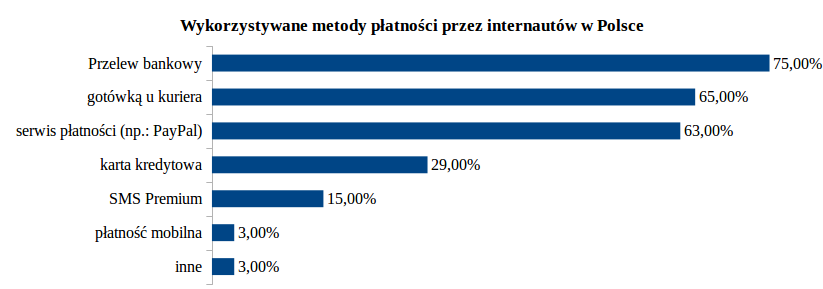
\includegraphics[width=1\linewidth]{01/popularnosc_platnosci}
	\end{center}
	\caption{Płatności z których korzystają internauci}
\end{figure}

%TODO napisać o nich może więcej, dokłądniej. Nazwać to Systemy Płatności, wyjaśnić te wszsytkie nazwy. ie będzie pewnie wiele dłuższe, no ale to jest w tytule
\subsection{Bramki płatności}
% co to jest. Opowiedzieć o związku z portfelami - ale że to inne pojęcia
% tutaj można dać jakiś diagramik jak to wszsytko wygląda
% opisać działanie
% zalety, dlaczego coś takiego stosować
% tabela z dostępnymi usługodawcami
Wdrożenie jednej lub kilku z wymienionych metod we własnym zakresie nie jest prostym rozwiązaniem. Implementacja z pominięciem wszelkich pośredników może okazać się zajęciem zbyt kosztownym i czasochłonnym, szczególnie dla firm rozpoczynających swoją działalność. Im więcej metod sprzedawca chce udostępnić, tym proces ten jest dłuższy i bardziej skomplikowany, angażując do tego kolejne podmioty. Wymaga to podpisania wielu dodatkowych umów z bankiem, czy posiadania specjalnego konta. 

Bardzo dobrą alternatywą jest skorzystanie z usług operatorów płatności elektronicznych. Są oni pośrednikami transakcji przeprowadzanych w internecie, przyjmując opłaty od klientów i przekazując następnie na rachunek sprzedawców. Ich usługi polegają na integrowaniu wielu metod płatności, dzięki czemu przedsiębiorca nie musi ręcznie wdrażać każdej z nich. Wystarczy, że podpisze umowę z jednym z dostawców systemów płatniczych. Jest to rozwiązanie korzystne także ze strony osoby dokonującej zakupów. Oferowany jest jej szeroki zakres metod, w jakich może dokonać płatności, np.: karty płatnicze, e-przelewy, portmonetki elektroniczne. Korzystanie z usług operatorów płatności jest bardzo częste. W popularnym polskim serwisie aukcyjnym Allegro, wszystkie opłaty realizowane są z pośrednictwem systemu PayU.

Przechodząc do finalizacji transakcji, klient proszony jest na stronie sprzedawcy o wybranie metody płatności. W przypadku przelewu internetowego, kierowany jest jeszcze na stronę swojego banku, skąd po podaniu danych, wraca na witrynę sprzedawcy. Po zaakceptowaniu zapłaty, operator usług dostaje przelew z banku klienta, skąd dalej w różny sposób pieniądze zostają przekazywane na rachunek sprzedawcy.
\begin{figure}[h]
	\begin{center}
		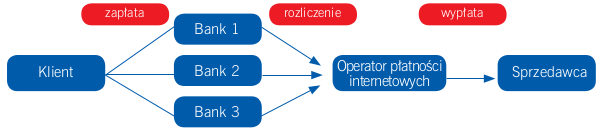
\includegraphics[width=1\linewidth]{01/diagram_system_platnosci}
	\end{center}
	\caption{Schemat działania bramek płatności}
\end{figure}
Na rynku istnieje wielu dostawców takich usług, np.: PayU, Dotpay, Przelewy24, czy PayPal. Różnią się oni między sobą przede wszystkim prowizjami za wypłatę pieniędzy, czy za skorzystanie z jakiejś metody płatności. Większość z nich pełni głównie rolę pośrednią, znajdując się między bankiem kupującego, a sprzedającego. Niektóre z nich, jak PayPal, pełnią także funkcję elektronicznych portmonetek. W tej sytuacji pieniądze od klienta nie trafiają do banku, a przechowywane są w formie elektroniczne. Sprzedawca decyduje czy i kiedy chce aby zostały one przelane na jego konto bankowe. 